\documentclass{article}
\usepackage{multicol}
\usepackage[ruled,vlined]{algorithm2e}
\usepackage{mathtools}
\usepackage[landscape,margin=0.2in]{geometry}

\usepackage{tikz}
\begin{document}
\begin{multicols*}{5}
		\section{Quake Heaps}
				Quake heaps are a collection of \textbf{tournament trees}, where the value at the parent node
				is the minimum of tha values at child nodes. Each node only has 1 or 2 children, and we can 
				have more than one tree side by side at the same time. 
				$\forall$ node, $h(x)=dis(x,$descendant node$)$. 

				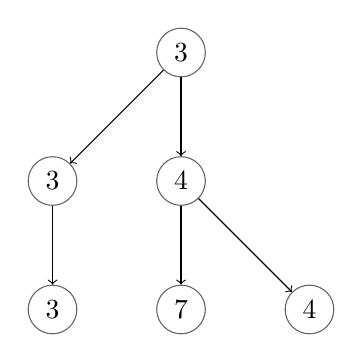
\begin{tikzpicture}[roundnode/.style={circle, draw=black!60},]
						\usetikzlibrary{positioning}
						\node[roundnode](maintopic){3};
						\node[roundnode](node1)[below=of maintopic]{4};
						\node[roundnode](node2)[left=of node1]{3};
						\node[roundnode](node3)[below=of node2]{3};
						\node[roundnode](node4)[below=of node1]{7};
						\node[roundnode](node5)[right=of node4]{4};

						\draw[->,black](maintopic) -- (node2);
						\draw[->,black](maintopic) -- (node1);
						\draw[->,black](node2) -- (node3);
						\draw[->,black](node1) -- (node4);
						\draw[->,black](node1) -- (node5); 
				\end{tikzpicture}
				Since every node has at most two children, then the height of each level $n_{i+1}$ will be 
				$\leq  \alpha n_{i}$, where $\alpha \in(1/2,1)$. Basically, every level will have 1/2-1 times 
				more nodes than the level directly downward. Its potential function is defined as 
				$N+T+B/(2\alpha-1)$, n=nodeNum, T=treeNum, B= deg-1 nodeNum. \textbf{Insert}$O(1)$, 
				\textbf{Dec-Key} $O(1)$,\textbf{Extract-Min} $O(\log n)$. When we Dec-Key, we remove the min 
				path from the top of tree to leaves in $O(\log n)$, then, we merge all the trees with height $i$. 

		\section{Disjoint Sets}
				A data structure that maintains collection of disjoint sets. 
				With \textbf{Make-Set(x)}, we create a singleton set $\{x\}$. With \textbf{Union(b,d)}, we make 
				a single set out of the two sets containing b and d respectively \textbf{Find-Set(x)} returns
				the \textbf{representative element} of set $S_{i}$. If DS doesn't change, then the RE will stay
				the same. 
				\subsection{Linked Lists}
					We can use LLs to maintain the data structure.  We maintain a pointer from avery element 
					to the representative, so $O(1)$ Find-Set(x). To merge two sets, we would need 
					$O(min(S1,S2))$.  It takes $O(n\log n + m)$ to perform seq. of m Make-Set(x), Find-Set(x),
					Union(x,y), in which ther eare n Make-Set(x) operations, due to the fact that we can update
					the pointers at least $O(\log n)$.
				\subsection{Forest Implementation}
					With this approach, we implement all the sets as a tree with elements pointing at the head. 
					Here, Union(x,y) takes $O(1)$ since we only update the root pointers when switching elements. 
					Just compare the size of the trees, adn append the larger one to the smaller one. However, 
					Find-Set(x) takes $O(h)$, where $h$ is the height of the tree. 
		\section{Graph Traversal}
					We can represent a graph by by using \textbf{adjacency list} or \textbf{adjacency matrix}. 
					There are differences in how much time it takes to check if there is a connection, vs. how 
					much space it takes to store a graph. The adjecency list might make it harder to iterate 
					and delete nodes, since it would have TC $O(\text{deg}(u))$

					\begin{algorithm}[H]
						\SetAlgoLined	
							visited[1..n] =$\{\text{no}\}$\;
							dis[1..n] = $\{\inf\}$\;
							parent[1..n] = $\{NIL\}$\;

							EnQueue(Q,s)\;
							\While{Q$\neq$0}
							{
								u = DeQueue(Q)\;			
								\For{ v$\in$Adj$[u]$ }
								{
										\If{visited$[v]$=no}
										{
											EnQueue(Q,v)\;			
										}

								}
							}
							\caption{BFS(G,S)}	
					\end{algorithm}
							For this algorithm, all the nodes are enqueued at most once, since their visited field
							is changed when enqueued. Therefore, it takes $O(n+m)$
				\subsection{Applications}
							The \textbf{diameter} of a tree is the maximum distance between two nodes in the
							graph. If we run BFS(T,c) and record the node with largest $d$: this is $o_{1}$ 
							or $o_{2}$. There are 4 different cases.
				\subsection{DFS}
							For DFS, we keep visiting any previously unvisited nodes in G as soon as we find them.
							Then, we start to work on the node itself.  We mark them \textbf{white} if they 
							are not	discovered yet; \textbf{grey} if they have been discovered but are not
							finished; and \textbf{black} if they have been completely explored. However, it 
							will only discover the nodes reachable from the source node. 

							Proper DFS algo will call DFS-Visit() for multiple starting nodes, usually those that
							might not be reachable from previous starting nodes. 
							\begin{algorithm}[H]
								\SetAlgoLined
								time = time + 1\;
								u.d = time\;
								u.color = gray\;
									\For{all nodes $v \in$ Adj[u]}
									{
											\If{v.color == White}
											{
												v.parent = u\;			
												DFS-Visit(G,v)\;
											}			
									}
									u.color = Black\;
									time = time + 1\;
									u.f = time\;
								\caption{DFS-Visit(G,u)}
							\end{algorithm}
			\subsection{Parenthesis Theorem}					
					For any two nodes $u$ and $v$, exactly one of the following holds: 
					\begin{itemize}
							\item{The intervals [u.d, u.f] and [v.d, v.f] are disjoint}
								neither is a descendant of the other. 
							\item{The interval [v.d, v.f] contains the interval [u.d, u.f]}
									:v is an ancestor of u
							\item{The interval [u.d,u.f] contains the interval[v.d,v.f]}: 	
									u is an ancestor of v. 
					\end{itemize}
					There are four different types of edges:
					\begin{itemize}
							\item{\textbf{tree edges}}: v discovered while v.color == white
							\item{\textbf{back edges}}: while exploring (u,v), v.color == Gray
							\item{\textbf{forward edges}}: while exploring (u,v), v.color == black and
									u.d < v.d 
							\item{\textbf{cross edges}}: while expl.(u,v), v.color == black and u.d>v.d
					\end{itemize}
			\subsection{Topological Sort}
				TS is an ordering of nodes so that for each edge (u,v), node u appears earlier than v in the 
				ordering. The algorithm involves performing DFS and adding the discovered node to the front
				of a list every time we finish exploring it. 
\end{multicols*}
\end{document}
